\documentclass[12pt]{article}
\usepackage{graphicx}
\usepackage {color}
\usepackage{pdfpages}
\usepackage{float}
\usepackage{changebar}
\usepackage{enumitem,amssymb}
\renewcommand{\familydefault}{\sfdefault}
\usepackage[margin=1.2in]{geometry}
\usepackage{graphicx}
\usepackage{wrapfig}
\usepackage[super]{cite}
\usepackage{subcaption}
\usepackage[table]{xcolor}
\usepackage{amsmath}
\usepackage[sort, numbers]{natbib}
\usepackage{multirow}
\usepackage{tabularx}
\usepackage{siunitx}

%%%%%%%%%%%%Defining the margins %%%%%%%%%%%%%%%%%%%%%
\textheight 9.in
\textwidth 6.5in
\topmargin -.5in
\oddsidemargin 0in
\setlength{\parskip}{\smallskipamount}

%%%%%%%%%%%%%%Specific Commands %%%%%%%%%%%%%%%%%%
\newcommand{\eg}{{\em e.g.,}}
\newcommand{\ie}{{\em i.e.,}}
\newcommand{\etc}{{\em etc.,}}
\newcommand{\etal}{{\em et al.}}
\newcommand{\degrees}{{$^{\circ}$}}
\newcommand{\fig}[1]{Figure~\ref{#1}}
%%%%%%%%%%%%%%%%%%%%%%%%%%%% Setting to control figure placement
% These determine the rules used to place floating objects like figures 
% They are only guides, but read the manual to see the effect of each.
\renewcommand{\topfraction}{.9}
\renewcommand{\bottomfraction}{.9}
\renewcommand{\textfraction}{.1}
\renewcommand{\familydefault}{\sfdefault} %setting the san serif font

%%%%%%%%%%%%%%%%%%%%%%%% Line spacing
% Use the following command for ``double'' spacing
%\setlength{\baselineskip}{1.2\baselineskip}
% and this one for an acceptable NIH spacing of 6lpi based on 11pt
%\setlength{\baselineskip}{.9\baselineskip}
% The baselineskip does not appear to work when we include a maketitle
% command in the main file.  Something there must set the line spacing
% If we use this next command, then things seem to work.
\renewcommand{\baselinestretch}{.9}
\newcommand{\coo}{CO$_2$}
\newcommand{\oo}{O$_2$}
\newcommand{\spo}{SPO$_2$}
\setcounter{secnumdepth}{0} %make no numbers but have a table of contents


\begin{document}

\title{Lab 6: Spriometry and Respiratory Regulation}
\author{Jake Bergquist, u6010393, Partner: Bram Hunt }
\maketitle

\section{Introduction}
The purpose of this laboratory exercise was to examine the various mechanism of respiration, how the various volumes and phenomena can be measured, and how the respiratory system responds to changes via various stimulus. In particular we sought to investigate the control of the respiratory system and the response of the respiratory system control to changes in base metabolism rate, oxygen in the air, carbon dioxide in the air, and dead space. 

The respiratory system is principally controlled by in voluntary autonomic systems in the nervous system. These systems are driven by receptors that sense the chemical balance in the blood and cerebro spinal fluid with respect to oxygen concentration, carbondioxide concentration, and pH, as well as mechanical receptors that sense the distension of the chest during respiration. The breathing cycle is mainly determined by inspiration rate. Expiration signals are constantly sent and periodic inspiration signals override the expiration stimulus. Inspriatory signals are unregulated by a decrease in oxygen concentration in the blood, and an increase in carbondioxide concentration in the blood and cerebro spinal fluid (which corresponds to a decrease in pH). These chemical changes are sensed by chemical sensing cells in the aortic arch and carotid arteries. By contrast, deep or rapid inspiratins result in stimuli from stretch receptors that would inhibit inspiration. Because there are many signals that must be integrated to regulate autonomic breathing this regulation must be controlled centrally at the brain stem, specifically the medulla oblongata. There is of couyrse manual override of breathing control, but the scope of this manual control is limited. Of the stimuli that affect the rate of respiration, the concentration of carbondioxide in the blood is the strongest effector, even more so than oxygen concentration. While some of these biochemical regulation methods are not fully understood, it is known that carbondioxide is directly related tot he pH buffering of the blood, as carbondioxide dissolves into carbonic acid int he blood which is essential to the blood pH buffering system. Additionally the cerebro spinal fluid is poor;ly buffered and thus its pH can be affected greatly by changes in carbondioxide concentration.

Metrics of breathing usually involve measuring several different respiratory volume. Such volumes like tidal volume, which measures the volume of air moved during rest breathing, as well as expiratory reserve (volume of breath that can be expired after a rest expiration), inspiratory reserve (volume of air that can be inspired after a rest inspiration), vital capacity (volume that can be expired after a maximum inspiration), residual volume (volume of air that cannot be expired), total lung capacity, and dead space (amount of air that does not move during respiration), are all used to diagnose various respiratory conditions. During this laboratory exercise we investigated all of these volumes as well as changes to respiration by various stimuli.

\section{Methods}

\subsection{Spirometry}
The spirometer used was calibrated using a known volume of air pressed into the device. Several values of known volume were used and the deflection in mV seen on the recording equipment was recorded. These volumes and changes in voltage were used to determine a conversion factor from mV to mL of air moved. The subject was then instructed to breath at rest into the device, followed by a maximal inspiration, a maximal forced expiration, and again normal breaths. With these breathing patterns we were able to calculate all the necessary lung volumes.

\subsection{Respiratory Rate}
We then examined respiratory rate under the condisitions of rest, mild exercise, and increased dead space. Heart rate and starting SPO$_2$ were measured followed by a minute of breathing rate recording. This was done at rest, after a brief run around the building, and again at rest but the subject was breathing through three feet of tubing. The three feet of tubing add dead space to the subject's respiratory system.

\subsection{Breath Holding}
The subject was then asked to hold breath as long as possible at rest, after hyperventilation, and after exercise.

\subsection{Physical Models}
We then investigated a couple of physical models of alveolar filling. We investigated filling one balloon of the alveolar model more than the other then letting their pressures interact. We then used a lung model to observe the filling of the lungs under different pressure scenarios.

\subsection{Re-Breathing}
We then allowed the subject to re-breath air under two conditions, CO$_2$ scrubbing and O$_2$ rich. Under \coo{} conditions the air  that the subject was re-breathing was had the \coo{} removed constantly while the \oo{} was allowed to be metabolized normally. In the \oo{} trial an excess of \oo{} was sent into the system and the \coo{} was allowed to accumulate naturally. During each trial the subject rebreathed the air while breath rate, inspired and expired \coo{} and \oo{}, heart rate, and SPO$_2$ were measured. The trial was terminated if the patient became too uncomfortable, or if SPO$_2$ fell too low or \coo{} concentrations rose too high.

\section{Results}
\subsection{Spirometry}
 The spirometry results are summarized with an example plot in Figure~\ref{fig:Vols} and the measurements in Table~\ref{tab:vols}. When compared tot he measurements taken by the dedicated FEV$_1$ device we find agreement with out measurements. The device showed a FEV$_1$ of 3.54 Liters (3540 mL) which agrees with our measured volume of 3.095 L. when compared to documented volumes of Wikipedia we find some agreement. It is stated in the Wikipedia article we were instructed to compare against that the volumes are typically larger in taller persons, at higher altitude, and when he subject is fit. In our case our subject is over 6 ft tall, lives at moderately high elevation, and is fit. This explains why the volumes we record are larger than expected. The only exception is inspiratory capacity which is reported at 3.5 Liters, which is close to our measured value of 3.639 Liters.

\begin{figure}[H]
	
	\centering
	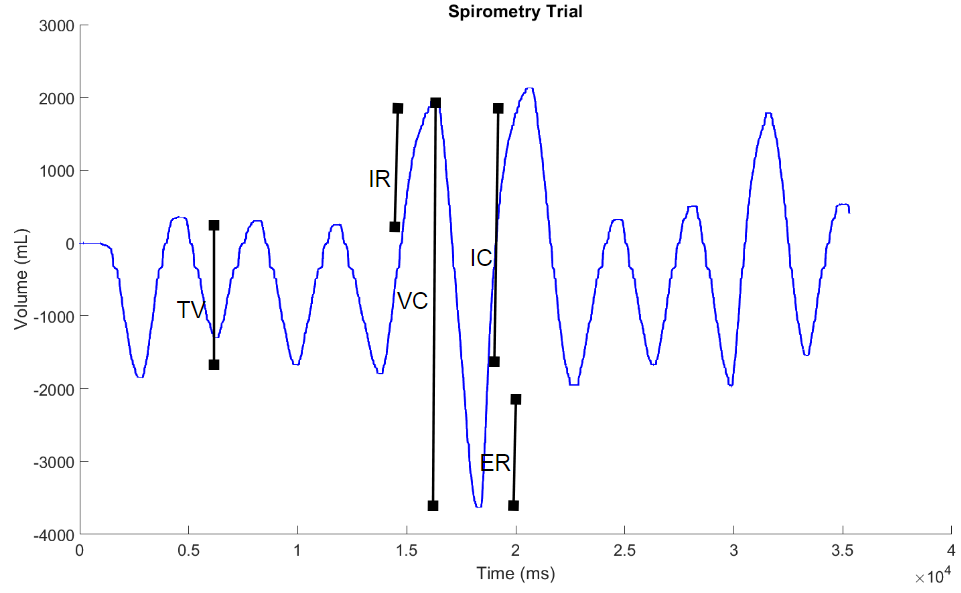
\includegraphics[width = .8\textwidth]{Figures/BreathVols.png}
	\caption{Sample of breath volume measurement trial. Shown are measures of tidal volume (TV), inspiratory reserve (IR), vital capacity (VC), inspiratory capacity (IC), and expiratory reserve (ER).}
	\label{fig:Vols}
\end{figure}

\begin{table}[H]
	\centering{}
	\caption{Breaths per minute under exercise, rest, and added dead space conditions. }
	\label{tab:vols}
	\begin{tabular}{|r|r|r|}
		\hline
		& Volume (mL) & STD (mL)\\
		\hline
		
		TV&1965 & 216 \\
		\hline
		IR&1673 & 259 \\
		\hline
		ER&1976 & 331 \\
		\hline
		IC&3639 & 125 \\
		\hline
		VC&5615 & 264 \\
		\hline
		FEV$_1$&3095 & 258 \\
		\hline
		
		
	\end{tabular}
\end{table}

\subsection{Respiratory Rate}
The numerical results for the breaths per minute trials are shown in Table~\ref{tab:bpm}. The two rest periods did not result in different numbers and are displayed together. During the extra dead space trial where the subject was breathing through the tube an increased depth of breathing was noted. The breathing seemed more labored and was much deeper than at rest.
\begin{table}[H]
	\centering{}
	\caption{Breaths per minute under exercise, rest, and added dead space conditions. }
	\label{tab:bpm}
	\begin{tabular}{|r|r|r|r|}
		\hline
		& Breath Per Minute & Start HR & Start \spo{} \\
		\hline
		
		Rest&14 & 84 &96\\
		\hline
		Exercise&17 & 151 &98\\
		\hline
		Extra Dead Space&7 & 101 &98 \\
		\hline
		
		
	\end{tabular}
\end{table}


\subsection{Breath Holding}

The numerical results from the breath hold trial are shown in Table~\ref{tab:bhold}. As can be seen the subject struggled to hold their breath after exercise.

\begin{table}[H]
	\centering{}
	\caption{Breath hold measurements. Time given in seconds. Start HR and \spo{} taken right before breath hold initiated. End \spo{} and HR taken when breath hold terminated. During exercise trial the heart rate was too high to measure well ont he pule oximeter. }
	\label{tab:bhold}
	\begin{tabular}{|r|r|r|r|r|r|}
		\hline
		 & Time (s) & Start HR & Start \spo{}&End HR & End \spo{} \\
		\hline
		
		Rest&75 & 101 &98 & 88 & 96\\
		\hline
		Hyperventilate&105  & 101 &98 & 91 & 98\\
		\hline
		Exercise&8 & too high &69 & too high & 94\\
		\hline
		
		
	\end{tabular}
\end{table}

\subsection{Physical Models}
When using the alveolar two balloon model we found that inflating one balloon more than the other then allowing the pressures to interact resulted in the less inflated balloon becoming even less inflated and the more inflated balloon becoming more inflated. With the lung model we found that when we pulled on the `diaphragm' and released the volve the balloons inflated.


\subsection{Re-Breathing}

The rebreathing of carbondioxide scrubbed vs oxygen rich air are shown in the following figures. Figure~\ref{fig:R1} shows the paprameter measurements from \coo{} scrub rebreathing while Figure~\ref{fig:R2} shows the instantaneous tidal volume during this trial. As can be seen the tidal volume did not change much. The subject did not report any distress during this trial despite the continuous decrease in \spo{} and \oo{} concentration. By contrast during the oxygen rich trial the subject reported difficulty breathing. These results are shown in Figure~\ref{fig:O1} and Figure~\ref{fig:O2}. Here we see an increase in instantaneous tidal volume as the \coo{} concentration increases as well as a slight increase in HR. All this despite no change in \spo. In both trials the breats per minute tracking was occasionally faulty and thus is missing some time instants.

\begin{figure}[H]
	
	\centering
	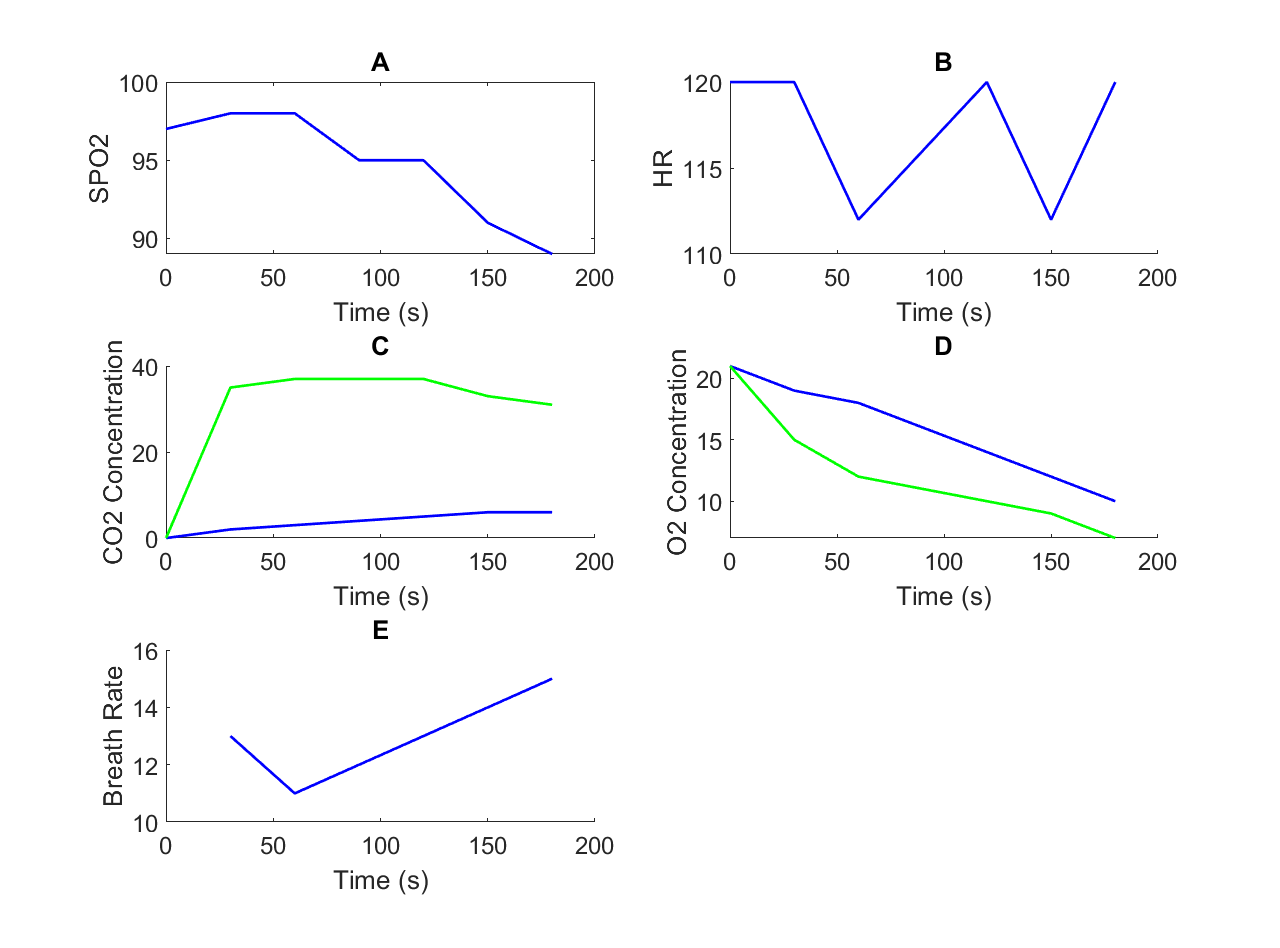
\includegraphics[width = .8\textwidth]{Figures/room_1.png}
	\caption{Measurements from rebreathing room air with \coo{} scrub. \spo{} over time (a), heart rate (B), inspired \coo{} (C, blue), expired \coo{} (C, green), inspired \oo{} (D, blue), expired \oo{} (D, green), breathing rate (E). }
	\label{fig:R1}
\end{figure}

\begin{figure}[H]
	
	\centering
	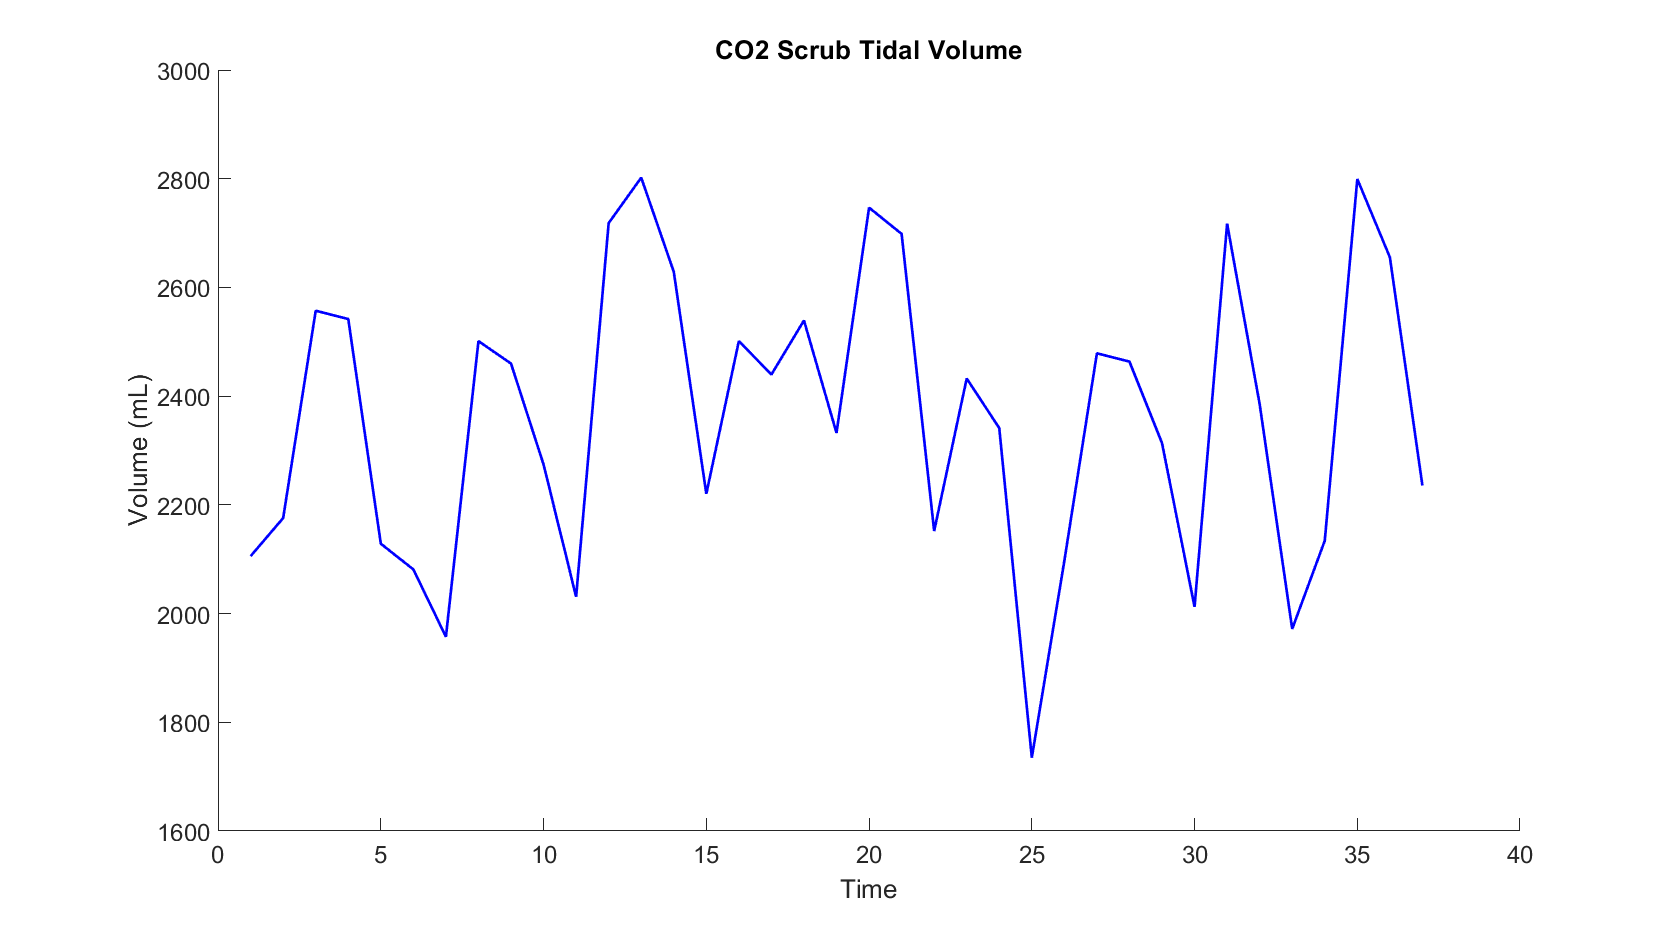
\includegraphics[width = .8\textwidth]{Figures/room_2.png}
	\caption{Tidal volume over time during the room air with \coo{} scrub rebreathing. Time instants represent one breathing cycle.}
	\label{fig:R2}
\end{figure}

\begin{figure}[H]
	
	\centering
	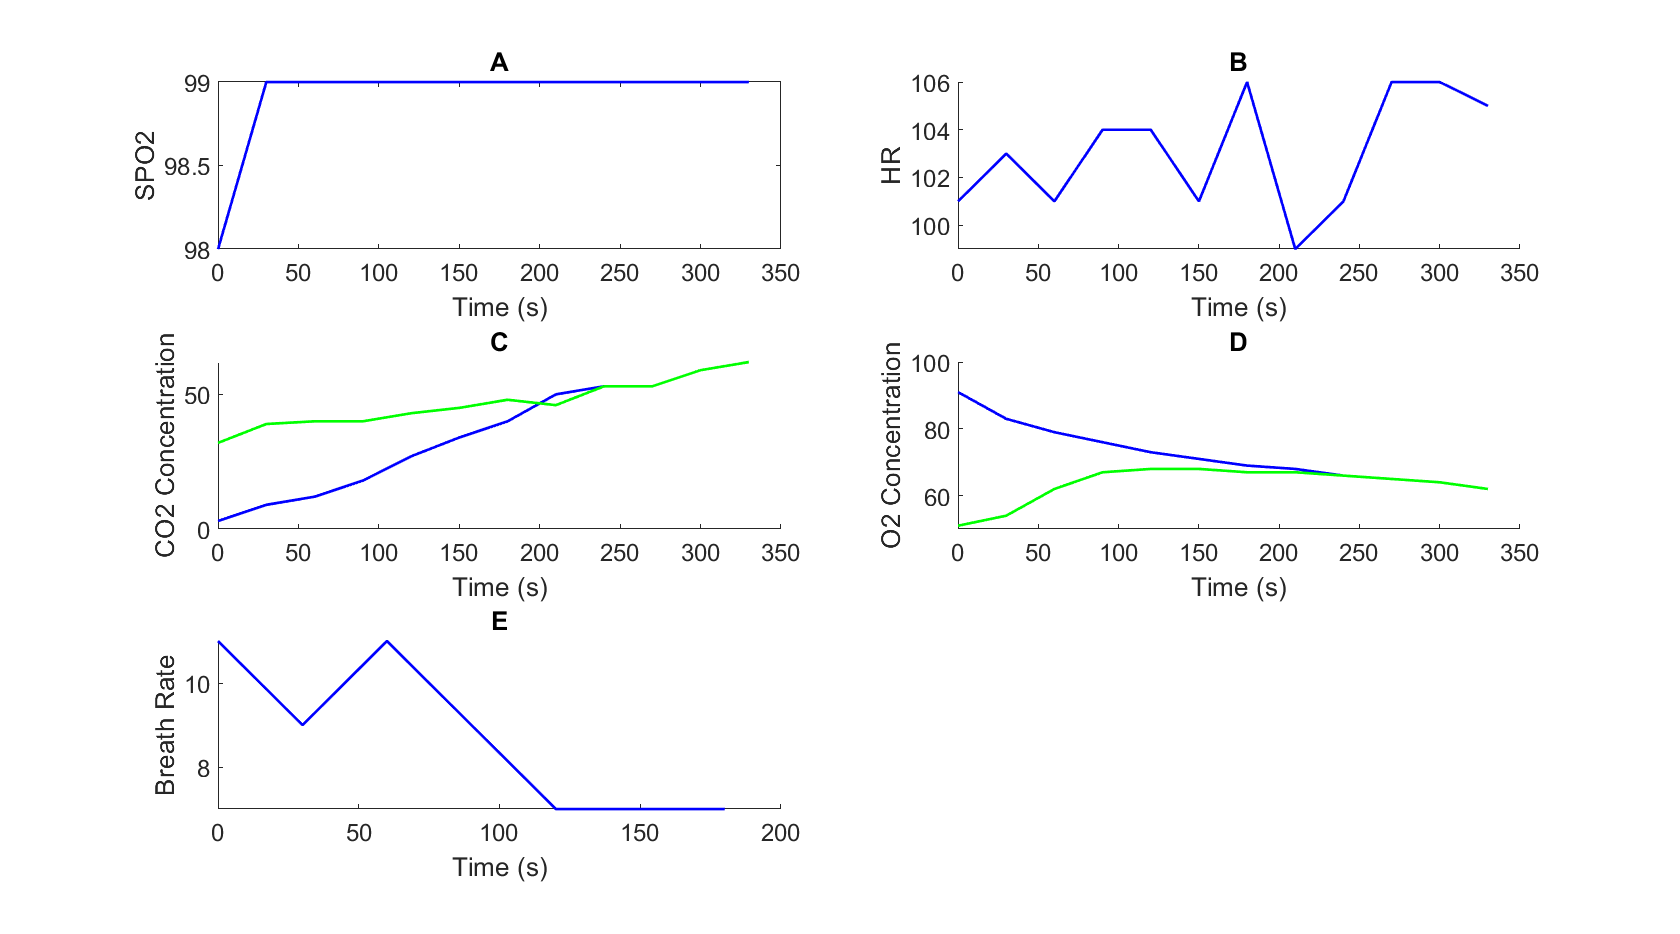
\includegraphics[width = .8\textwidth]{Figures/Higho2_1.png}
	\caption{Measurements from rebreathing high oxygen concentration air. \spo{} over time (a), heart rate (B), inspired \coo{} (C, blue), expired \coo{} (C, green), inspired \oo{} (D, blue), expired \oo{} (D, green), breathing rate (E).}
	\label{fig:O1}
\end{figure}

\begin{figure}[H]
	
	\centering
	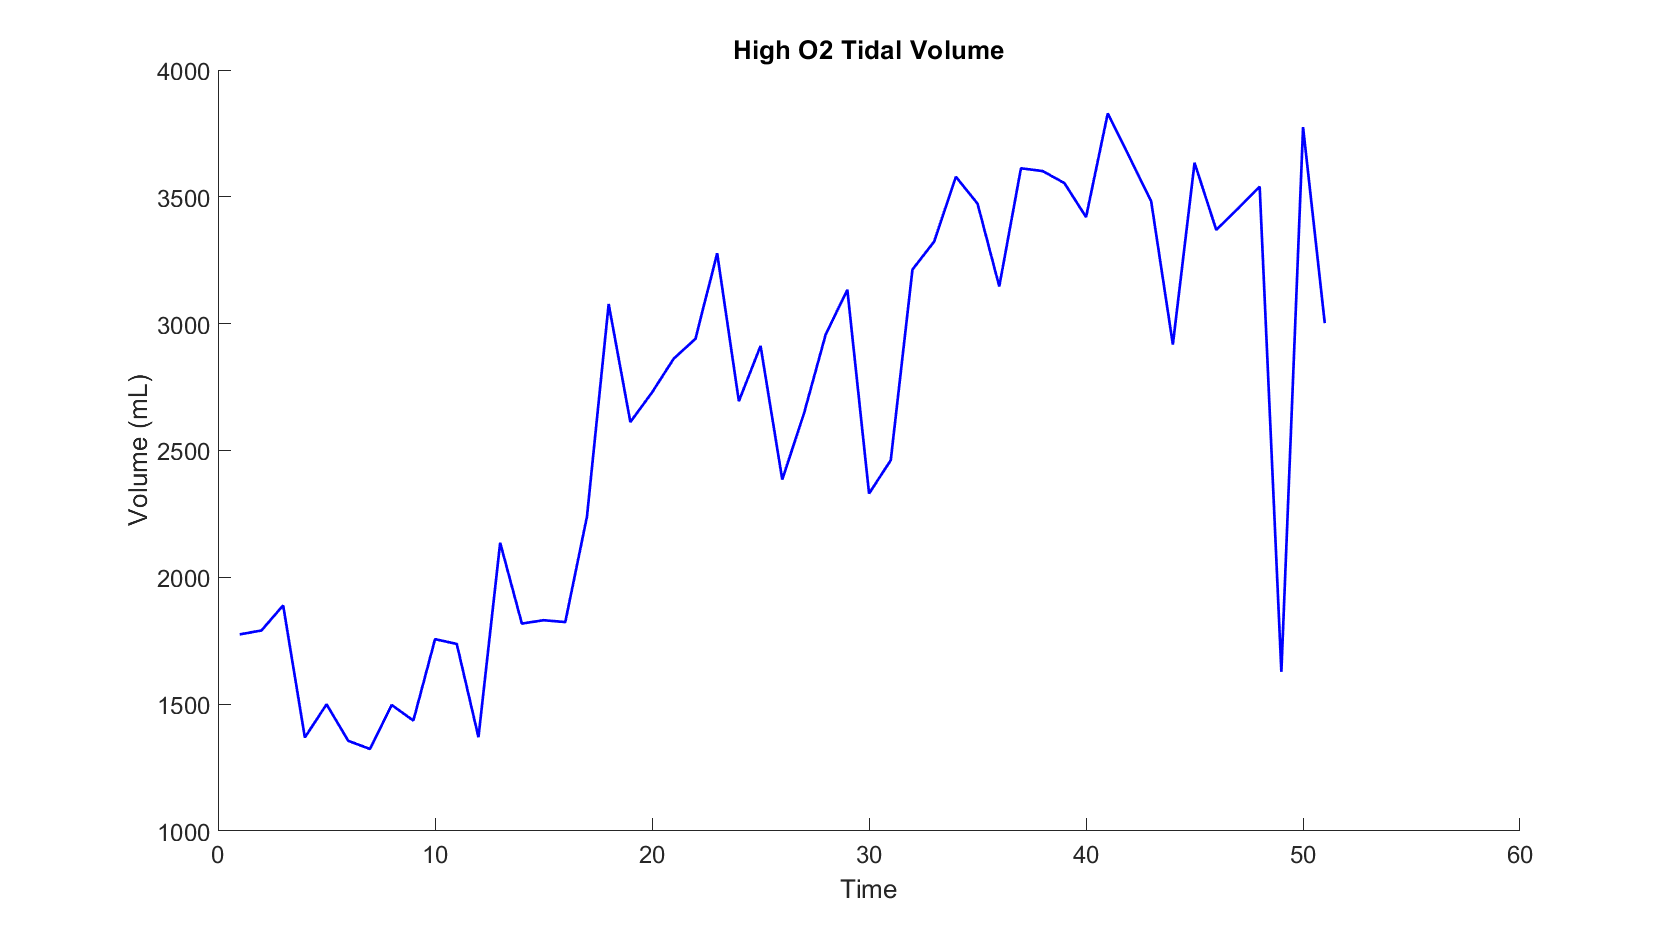
\includegraphics[width = .8\textwidth]{Figures/Higho2_2.png}
	\caption{Tidal volume over time during the high oxygen concentration rebreathing. Time instants represent one breathing cycle.}
	\label{fig:O2}
\end{figure}

\section{Discussion}

\subsection{Spirometry}
During this section we measured the specific lung volumes of the subject (Table~\ref{tab:vols} and Figure~\ref{fig:Vols}). We found that these volumes generally tended to be larger than expected reported volumes, however given that the subject is over 6ft tall and lives at high altitude this makes sense. Larger bodies result in larger lungs, and at higher altitude a larger volume of air flow is necessary to maintain proer blood gas exchange. During the  measure of FEV$_1$ we found that both the direct spirometry measure and the ddedicated device measure produced similar results (3.095 L and 3.54 L respectivly). Measuring FEV$_1$ is important for understanding the health and functioning of the lungs. A lowered FEV$_1$ indicates pulmonary obstructions or other diseases that affect the lung's ability to move air. 

\subsection{Respiratory Rate}
During this trial the subject was allowed to breath freely and the rate of breathing as well as any other qualitative measures were made during rest, post exercise, and with additional dead space added. At rest the subject showed a basal breaths per minute of 14 (Table~\ref{tab:bpm}) This jumped to 17 post exercise with an elevated heart rate of 151 beats per minute. To add extra dead space to the system the subject was instructed to breath through a 3 ft length of tubing. It was important that this tubing be exposed to open air to not confound these results with the processes present when the subject rebreaths room air. The subject needed to be breathing, not rebreathing, so that \coo{} concentrations would not increase and \oo{} concentrations would not decrease. These factors would likely confound our analysis of the additional dead space. While it is true that using the spirometer also adds dead space due to the tubing, these other confounding factors lead us ot use a simple open ended tube. During this trial the breaths per minute dropped dramatically  to 7 while the breaths themselves became much deeper and labored. The subject reported difficulty breathing. This is likely due to the extra effort needed to breath with extra dead space. The increase volume of breaths was also due to the increased dead space, and these increased volumes of breaths resulted in decreased breathing rate due to negative feedback by stretch receptors in the chest.

\subsection{Breath Holding}
During this trial the subject was instructed to hold their breath as long as possible at rest, after exercise, and after hyperventilating. At rest this time was 75 seconds with a basal heart rate of 101 beats per minute, and \spo{} of 98. Post breath hold the heart rate had dropped to 88 beats per minute while the \spo{} did not change much (Table~\ref{tab:bhold}). The reduction in heart rate is directly related to the reduction in respiration. After hyperventilation the subject was able to hold their breath much longer, up to 105 seconds. Again we saw a similar drop in heart rate during the breath hold. Hyperventilation over-oxygenates the blood and drives off excess \coo{}, thus the urge to breath is delayed by the reduced \coo{} concentration int he blood. After exercise the subject was hardly able to hold their breath at all, only managing 8 seconds. This makes sense as the metabolic demand by the body high such that the urge to breath overrides the conscious control of the breathing.

\subsection{Physical Models}
During the examination of the physical models of the lung we found that by inflating one alveolar balloon to a higher extent than the other and allowing the pressures to interact we saw the more inflated balloon became even more inflated while the less inflated balloon became less inflated. This relates to the material properties of the balloons and similarly to the alveolar sacs. The more stretched balloon is more compliant while the less stretched one requires more energy to induce any more stretch. This is important to understand int he lungs as it implies that the lungs must inflate uniformly to ensure that every alveolar sac is inflated properly. This is more easily accomplished in healthy tissue by negative pressure than forced positive pressure. The demonstration of the negative pressure lung model showed that when we applied a negative pressure by pulling of the diaphragm both `lung' balloons inflated equally.

\subsection{Re-Breathing}
The two rebreathing protocols produced different results both numerically and qualitatively. Despite the continuous decrease in oxygen concentration during the \coo{} scrub protocol, the subject did not report any trouble breathing or discomfort. We also did not see any change in heart rate or tidal volume indicating no mechanical changes in breathing were detected (Figure~\ref{fig:R1} and Figure~\ref{fig:R2}). However when ample \oo{} was provided but \coo{} was allowed to accumulate the subject reported difficulty breathing quickly, tidal volume increased, and heart rate slightly increased despite a contrant and high \spo. This phenomena while initially surprising, should be expected. We know that breathing regulation is primary driven by sensing of \coo{} levels rather than \oo{} levels. Thus when \coo{} is scrubbed, even though \oo{} falls to levels that would be problematic for the body it does not sense a problem, whereas when \oo{} is abundant but \coo{} is not cleared the breathing regulation systems sense a problem resulting in increased tidal volume, and a sensation of a need to breath or difficulty breathing.

Overall we found that, as expected, \coo{} is the principle driver of respiratory regulation as can be seen int he final experiments. A limitation of our study is the fact that the spirometers we used add a large amount of dead space to our subject's respiratory system. This could likely reflect int he increased tidal volumes we recorded as compared to literature values, and we have no good way of separating these effects from other explanations. Additionally we found that the pulseoximeter was limited especially post exercise in providing accurate measurements. To improve this we would likely utilize more direct measures such as an ECG and spirometry data as is done in a typical exercise lab.

%%%%%%%%%%%%%%%%%% Correct Bibliography Style

%\bibliography{C:/Users/Jake/Documents/library}
%\bibliographystyle{IEEEtran}


\end{document}








